%%%%%%%%%%%%%%%%%%%%%%%%%%%%%%%%%%%%%%%%%%%%%%%%%%%%%%
% A Beamer template for University of Wollongong     %
% Based on THU beamer theme                          %
% Author: Qiuyu Lu                                   %
% Date: July 2024                                    %
% LPPL Licensed.                                     %
%%%%%%%%%%%%%%%%%%%%%%%%%%%%%%%%%%%%%%%%%%%%%%%%%%%%%%
% Customized for Sharif University of Technology     %
%%%%%%%%%%%%%%%%%%%%%%%%%%%%%%%%%%%%%%%%%%%%%%%%%%%%%%


\documentclass[serif, aspectratio=169]{beamer}
%\documentclass[serif]{beamer}  % for 4:3 ratio
\usepackage[T1]{fontenc} 
\usepackage{fourier} % see 
\usepackage{caption}
\usepackage{hyperref}
\usepackage{latexsym,amsmath,xcolor,multicol,booktabs,calligra}
\usepackage{graphicx,pstricks,listings,stackengine}
\usepackage{lipsum}
\usepackage{outlines}
\usepackage{media9}

\author{Ali Sharifi-Zarchi}
\title{Machine Learning (CE 40717)}
\subtitle{Fall 2024}
\institute{
    CE Department \\
    Sharif University of Technology
}
%\date{\small \today}
% \usepackage{UoWstyle}
\usepackage{SUTstyle}
\usepackage[most]{tcolorbox}



% defs
\def\cmd#1{\texttt{\color{red}\footnotesize $\backslash$#1}}
\def\env#1{\texttt{\color{blue}\footnotesize #1}}
\definecolor{deepblue}{rgb}{0,0,0.5}
\definecolor{deepred}{RGB}{153,0,0}
\definecolor{deepgreen}{rgb}{0,0.5,0}
\definecolor{halfgray}{gray}{0.55}


\lstset{
    basicstyle=\ttfamily\small,
    keywordstyle=\bfseries\color{deepblue},
    emphstyle=\ttfamily\color{deepred},    % Custom highlighting style
    stringstyle=\color{deepgreen},
    numbers=left,
    numberstyle=\small\color{halfgray},
    rulesepcolor=\color{red!20!green!20!blue!20},
    frame=shadowbox,
}


\begin{document}

\begin{frame}
    \titlepage
    \vspace*{-0.6cm}
    \begin{figure}[htpb]
        \begin{center}
            
\includegraphics[keepaspectratio, scale=0.25]{pic/sharif-main-logo.png}
        \end{center}
    \end{figure}
\end{frame}

\begin{frame}    
\tableofcontents[sectionstyle=show,
subsectionstyle=show/shaded/hide,
subsubsectionstyle=show/shaded/hide]
\end{frame}

\section{Large Language Models}

\begin{frame}{Language models}
    \begin{itemize}
        \item 
            \large{Definition of a Language Model (LM)}
         \vspace{0.5cm}
        \begin{outline}
            \1 A machine learning model designed to predict and generate plausible language by analyzing text patterns.
            \vspace{0.2cm}
            \1 Operates by learning from large amounts of text data to understand linguistic structures, context, and vocabulary.
            \2 Common example: Autocomplete in text typing
        \end{outline}
    \end{itemize}
     
\end{frame}

\begin{frame}{Language models}
    \begin{itemize}
        \item  
            \large{Purpose of Language Models}
            \vspace{0.5cm}
            \begin{outline}
                \1 Estimate the probability of a word (token) or sequence of words within a longer text sequence.
                \vspace{0.2cm}
                \1 Aim to understand and predict context in sentences.
            \end{outline}
            \vspace{0.3cm}
        
    \end{itemize}
\end{frame}
    
\begin{frame}{Language models}
    \begin{exampleblock}{Example of Language Model Prediction}
        \begin{itemize}
            \item 
                When I hear rain on my roof, I \_\_\_\_\_\_\_ in my kitchen.\\
                Potential predictions with probabilities:\\
                \hspace{1cm}"cook soup" - 9.4\%\\
                \hspace{1cm}"warm up a kettle" - 5.2\%\\
                \hspace{1cm}"cower" - 3.6\%\\
                \hspace{1cm}"nap" - 2.5\%\\
                \hspace{1cm}"relax" - 2.2\%\\
        \end{itemize}
    \end{exampleblock}
\end{frame}

\begin{frame}{Language models}
    \begin{exampleblock}{The LLM Era – Paradigm Shift in Machine Learning}
        \hspace{2.8cm}
        \begin{figure*}
        \centering
        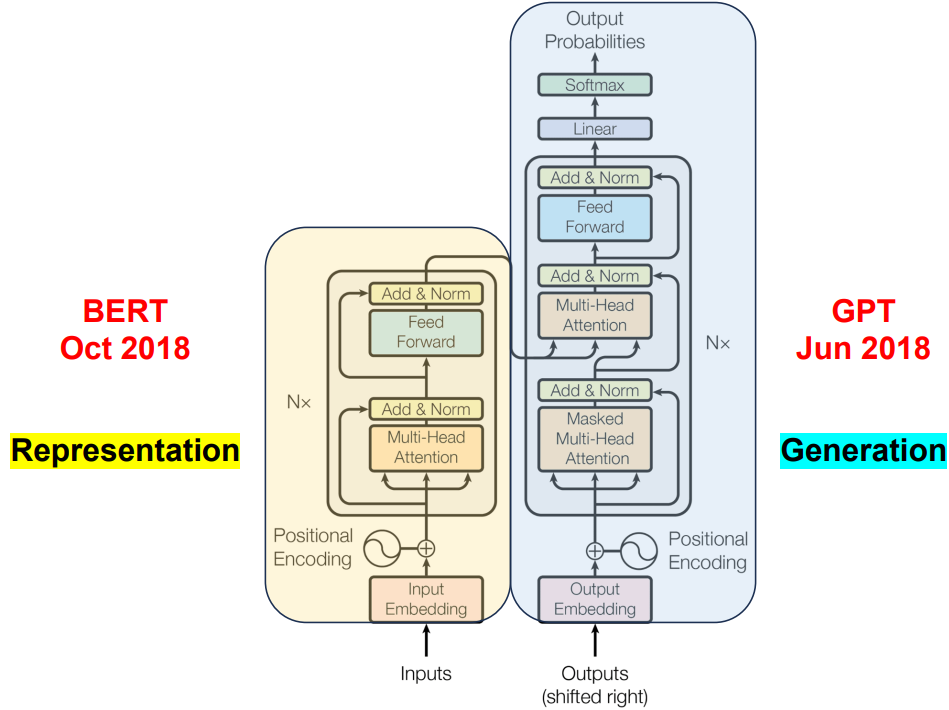
\includegraphics[width=0.6\textwidth]{pic/llm.png}
        \caption{}
        \end{figure*}
    \end{exampleblock}
\end{frame}

\begin{frame}{Generalizing to Unseen Tasks}
    \vspace{0.5cm}
    \begin{itemize}
        \item
            \large{LMs can be used for different tasks by pre-training a “base” model and then fine-tuning for the task(s) of interest}
            \vspace{0.3cm}
        \item 
            \large{Practical Issues:}
            \vspace{0.1cm}
            \begin{outline}
                \1 Too many copies of the model
                \1 Need for large-scale labeled data for fine-tuning
            \end{outline}
        \item 
            \large{Multi-task Training?}
            \vspace{0.1cm}
            \begin{outline}
                \1 Data remains a challenge 
                \1  Humans don’t need such large volumes of data to learn – can we do better?
            \end{outline}
        \item 
            \large{Train a model that can perform NLP tasks in a zero-shot manner}
    \end{itemize}
\end{frame}

\begin{frame}{Task Specifications}
    \vspace{0.5cm}
    \begin{itemize}
        \item
            \large{Primary shift comes from modeling assumptions from single-task to general model}\\
            \vspace{0.3cm}
            \hspace{2cm}
            \begin{figure*}
            \centering
            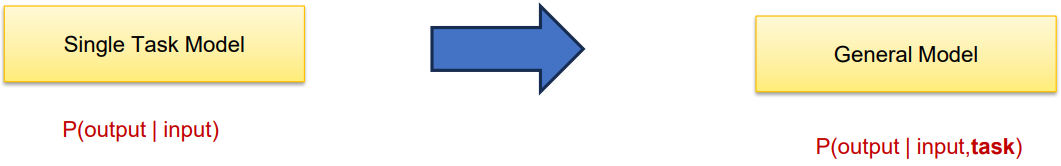
\includegraphics[width=0.7\textwidth]{pic/task specification.png}
            \caption{}
            \end{figure*}
        \item 
            \large{Task descriptions may be provided as text – for example, translate this French text to English}
    \end{itemize}
\end{frame}

\begin{frame}{Perplexity }
    \vspace{0.5cm}
    \begin{itemize}
        \item
            \large{Perplexity as a measure of uncertainty:} Perplexity is the exponentiation of the average negative log-likelihood of a probability distribution, representing the uncertainty of a model in predicting the next item in a sequence.\\
    \end{itemize}
    \vspace{0.5cm}
    \[
        \text{Perplexity}(P) = \exp\left( -\frac{1}{N} \sum_{i=1}^{N} \log P(w_i) \right)
    \]
    \begin{outline}
        \1 \( N \) is the number of words (or tokens) in the dataset,
        \1 \( P(w_i) \) is the probability of the \( i \)-th word in the sequence.
    \end{outline}
\end{frame}

\begin{frame}{Scaling}
    \vspace{0.5cm}
    \begin{itemize}
        \item
            \large{Scaling improves the perplexity of the LM and improves performance}\\
            \vspace{0.3cm}
            \hspace{2.8cm}
            \begin{figure*}
            \centering
            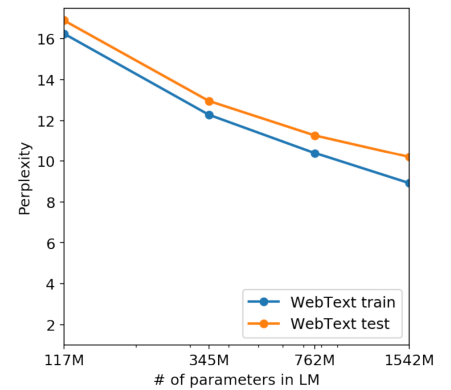
\includegraphics[width=0.4\textwidth]{pic/scaling gpt2.png}
            \caption{}
            \end{figure*}
    \end{itemize}
\end{frame}

\begin{frame}{Power-Law Scaling}
    \Large{Why is this interesting? Look at data scaling}
    \begin{itemize}
        \item
            \large{Loss and dataset size is linear on a log-log plot}\\
            \vspace{0.1cm}
        \item 
            \large{This is “power-law scaling”}
            \vspace{}
    \end{itemize}
    \hspace{2cm}
    \begin{figure*}
        \centering
        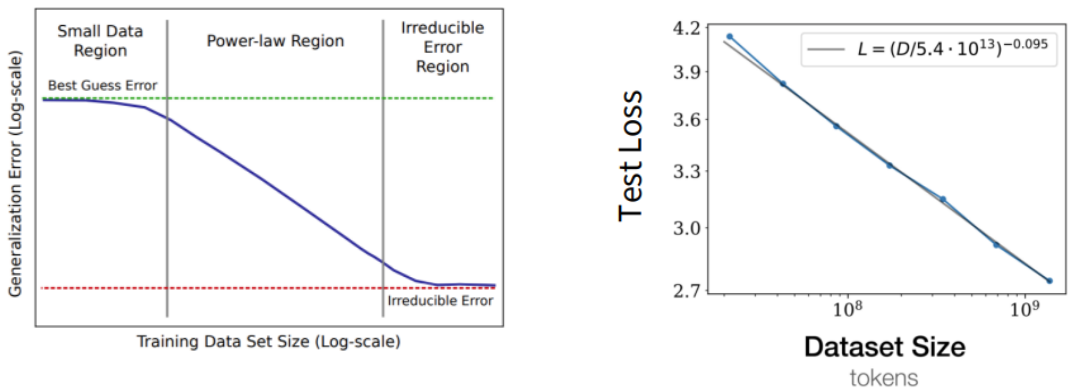
\includegraphics[width=0.75\textwidth]{pic/power low.png}
        \caption{}
    \end{figure*}
\end{frame}

\begin{frame}{NLP Moore's Law}
    \hspace{1.5cm}
    \begin{figure*}
        \centering
        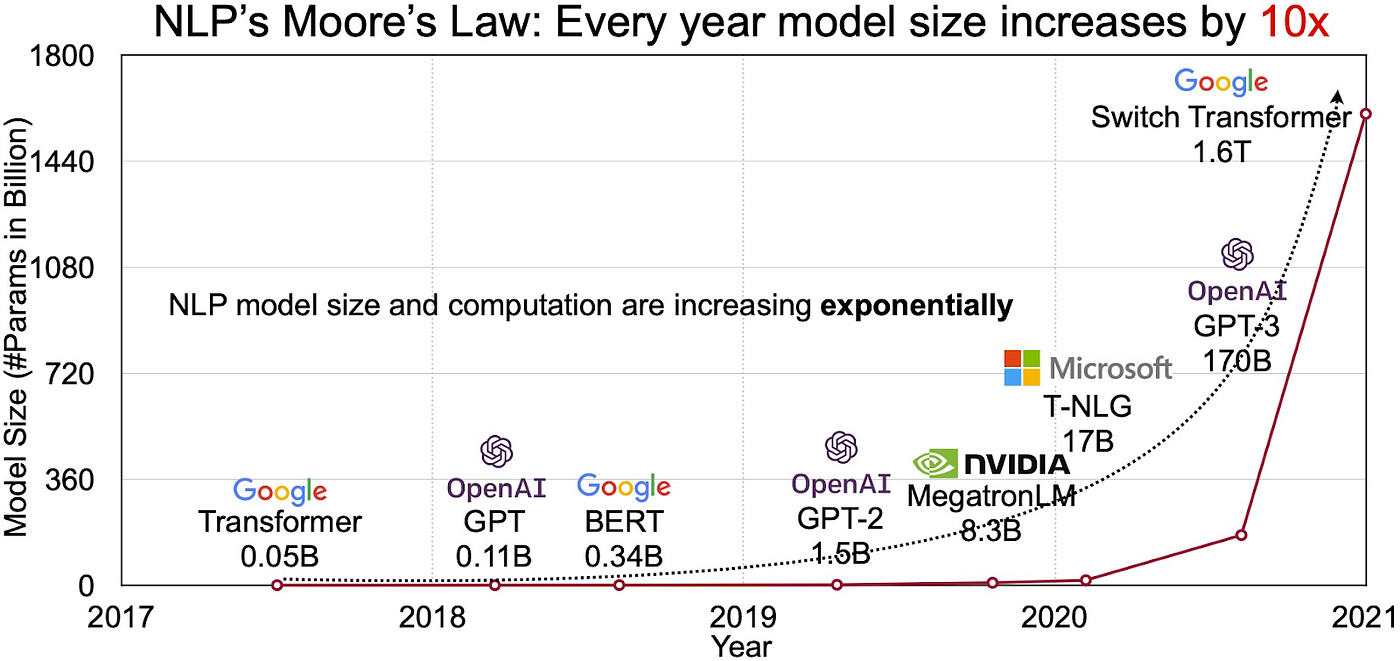
\includegraphics[width=0.75\textwidth]{pic/gpt3vs2.png}
        \caption{}
    \end{figure*}
\end{frame}

\begin{frame}{Large Language models}
    \begin{itemize}
        \item  
            \large{What are Large Language Models (LLMs)?}
            \begin{outline}
                \1 Large Language Models (LLMs) are advanced statistical models based on neural networks designed to process and generate natural language. Formally, an LLM can be defined as:
                \[
                P(w_1, w_2, \dots, w_N) = \prod_{i=1}^{N} P(w_i \mid w_1, w_2, \dots, w_{i-1})
                \]
                
                where:
                \begin{itemize}
                    \item \( w_1, w_2, \dots, w_N \) are words (or tokens) in a sequence,
                    \item \( P(w_i \mid w_1, w_2, \dots, w_{i-1}) \) represents the conditional probability of the \( i \)-th word given the previous words.
                \end{itemize}
            \end{outline}
            \item  
            \large{Key Characteristics of LLMs}
            \begin{outline}
                \1 \textbf{Architecture:} LLMs are typically built using Transformer-based architectures, where attention mechanisms are used to capture dependencies across the input sequence.
                \1 \textbf{Parameterization:} "Large" models have millions to billions of parameters (\( \theta \)), optimized using a loss function.
                \1 \textbf{Training:} Trained on massive text corpora with unsupervised tasks like next-word prediction or masked token prediction.
                \end{outline}
    \end{itemize}
\end{frame}

\begin{frame}{Generative Pre-Training (GPT)}
    GPT: Based on Transformer decoder layers\\
    \hspace{1.50cm}
    \begin{figure*}
        \centering
        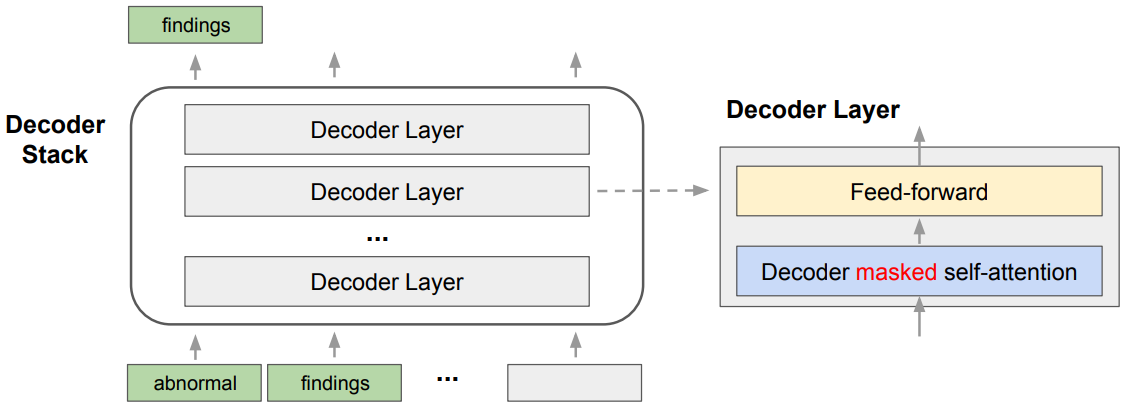
\includegraphics[width=0.9\textwidth]{pic/decoder only.png}
        \caption{}
    \end{figure*}
\end{frame}

\begin{frame}{GPTs}
    \hspace{2.90cm}
    \begin{figure*}
        \centering
        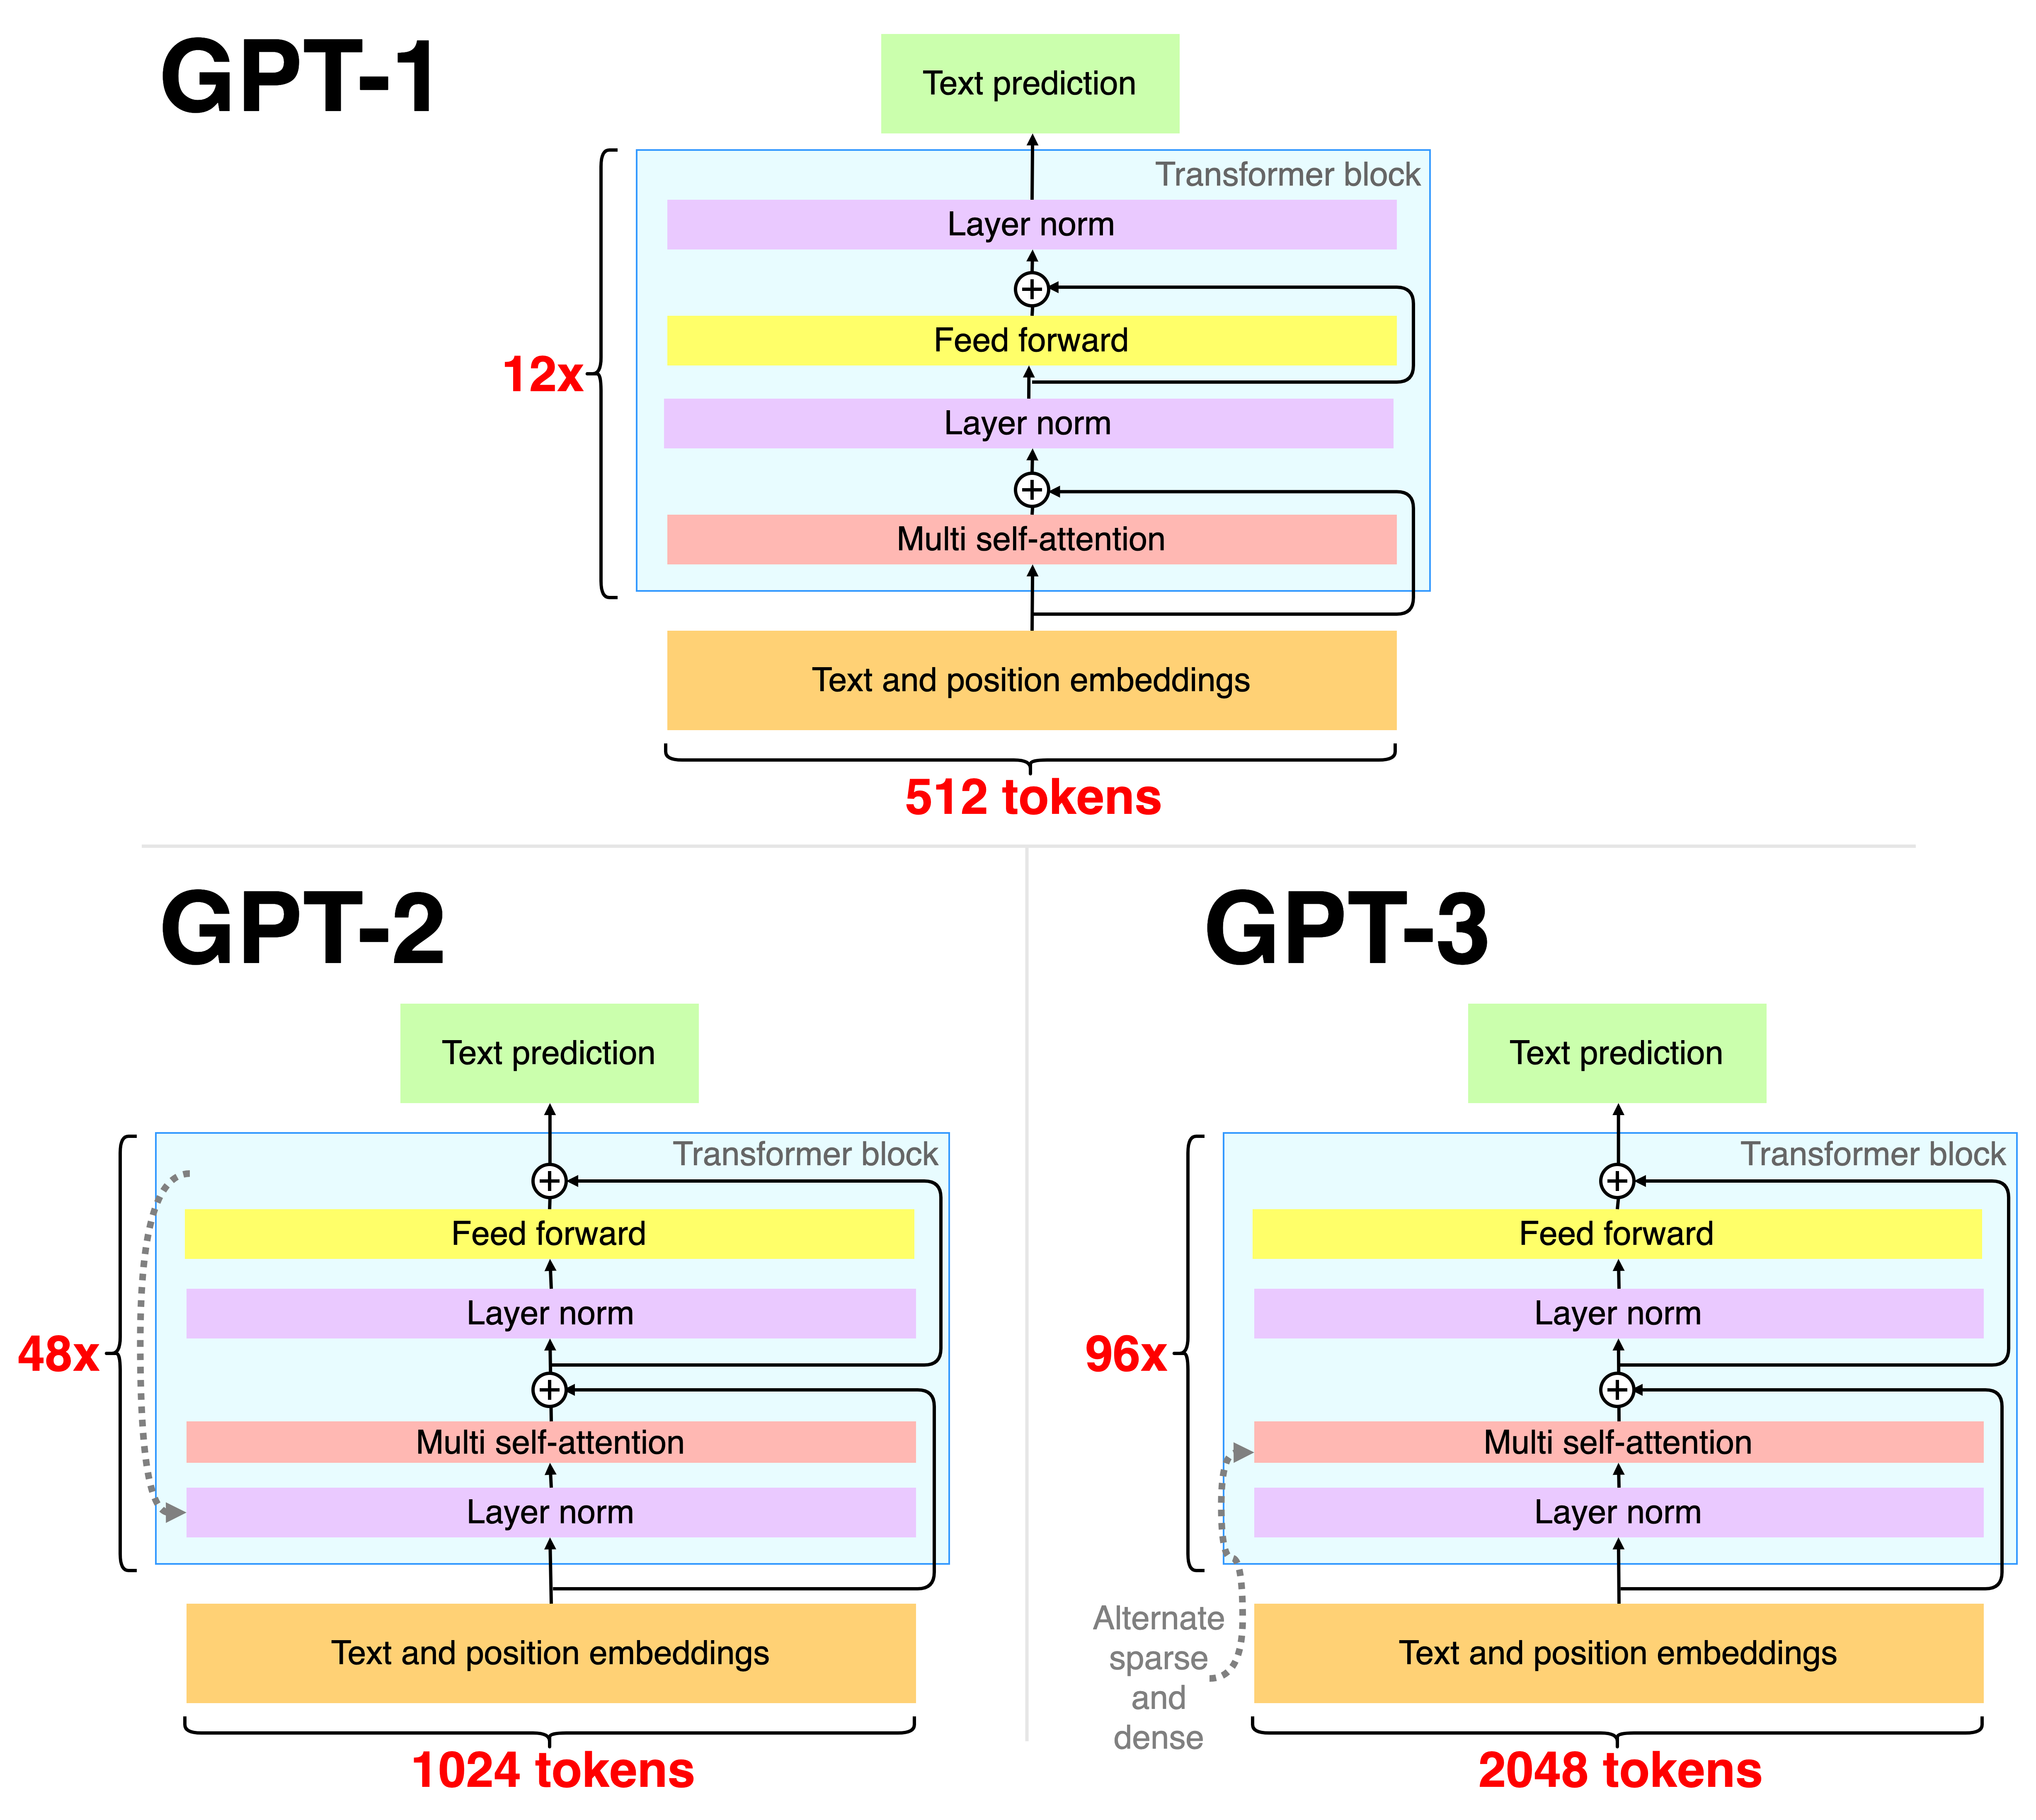
\includegraphics[width=0.55\textwidth]{pic/GPTS.png}
        \caption{}
    \end{figure*}
\end{frame}

\begin{frame}{GPT-2}
    \hspace{0.4cm}
    \begin{figure*}
        \centering
        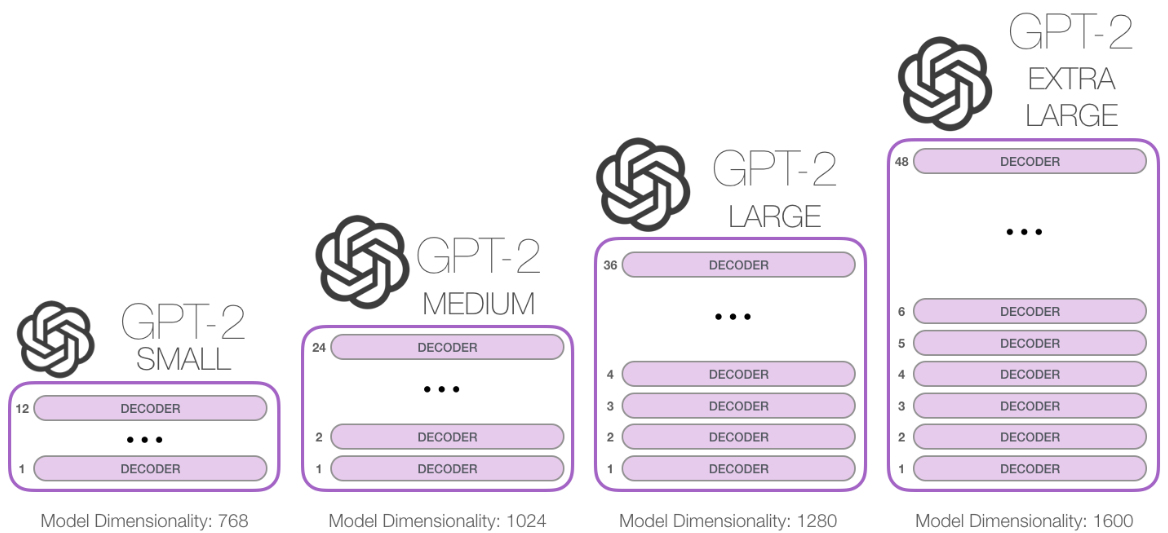
\includegraphics[width=0.99\textwidth]{pic/GPT-2.png}
        \caption{}
    \end{figure*}
\end{frame}

\begin{frame}{GPT-3}
    \hspace{0.4cm}
    \begin{figure*}
        \centering
        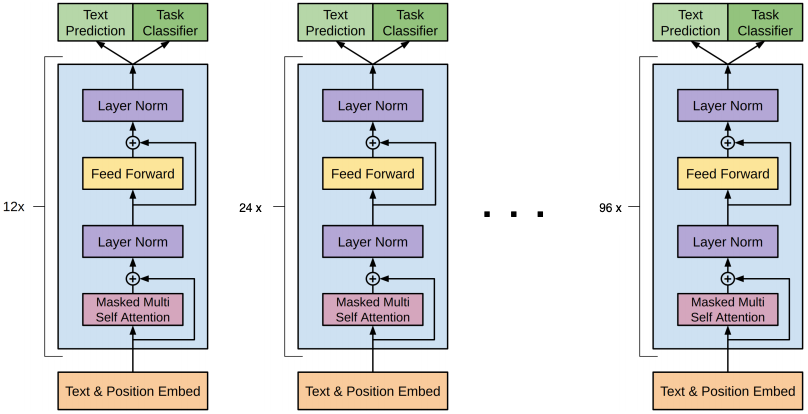
\includegraphics[width=0.95\textwidth]{pic/GPT-3.png}
        \caption{}
    \end{figure*}
\end{frame}

\begin{frame}{GPT-3}
    \Large{Emergent Abilities}
    \vspace{0.5cm}
    \begin{itemize}
        \item
            \large{Emergent abilities:}
                \begin{outline}
                    \1 not present in smaller models but is present in larger models
                    \1 Do LLMs like GPT3 have these ?
                \end{outline}   
            \vspace{0.1cm}
        \item
            \large{Findings:}
            \begin{outline}
                \1 GPT-3 trained on text can do arithmetic problems like addition and subtraction
                \1 Different abilities “emerge” at different scales
                \1 Model scale is not the only contributor to emergence – for 14 BIG-Bench tasks, LaMDA 137B and GPT-3 175B models perform at near-random, but PaLM 62B achieves above-random performanceb
                \1 Problems LLMs can’t solve today may be emergent for future LLMs
            \end{outline}
    \end{itemize}
\end{frame}

\begin{comment}
\begin{frame}{Large Language models}
    \Large{Architecture}
    \begin{itemize}
        \item  
            \large{Encoder-only (BERT)}
            \begin{outline}
                \1 Pre-training : Masked Language Modeling (MLM)
                \1 Great for classification tasks, but hard to do generation
            \end{outline}
            \vspace{0.3cm}
        \item 
            \large{Decoder-only (GPT)}
            \begin{outline}
                \1 Pre-training: Auto-regressive Language Modeling 
                \1 Stable training, faster convergence
                \1 Better generalization after pre-training
            \end{outline}
            \vspace{0.3cm}
        \item 
            \large{Encoder-decoder (T0/T5)}
            \begin{outline}
                \1 Pre-training : Masked Span Prediction
                \1 Good for tasks like MT, summarization 
            \end{outline}
    \end{itemize}
\end{frame}
\end{comment}

\begin{frame}{Attention patterns}
    \hspace{2cm}
    \begin{figure*}
        \centering
        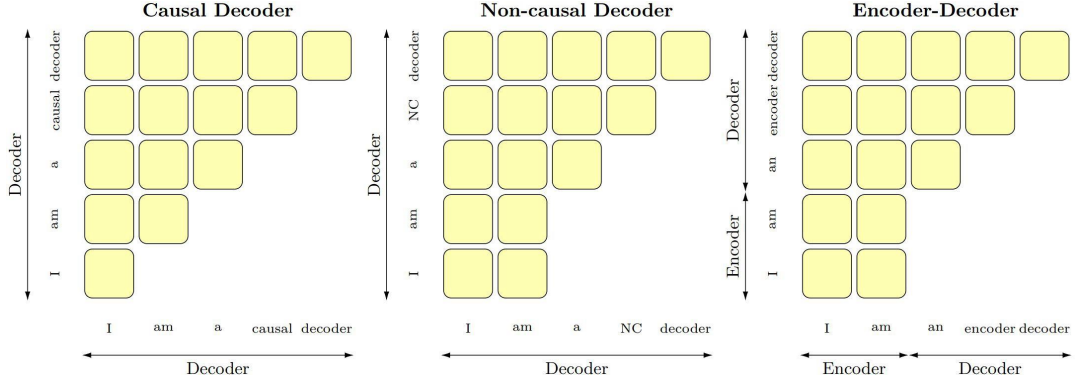
\includegraphics[width=0.7\textwidth]{pic/attention.png}
        \caption{}
    \end{figure*}
    \begin{itemize}
        \item Causal decoder -- each token attends to the previous tokens only. 
        \item In both non-causal decoder and encoder-decoder, attention is allowed to be bidirectional on any conditioning information.
        \item For the encoder-decoder, that conditioning is fed into the encoder part of the model. 
    \end{itemize}
\end{frame}


\begin{frame}{Llama 2 Architecture}
    \begin{itemize}
        \item Decoder-only model
        \item Changes in transformer module:
            \begin{outline}
                \1 Norm after sublayer -> Norm before sublayer
                \1 LayerNorm -> RMSNorm for stability
                \1 Activation: ReLU -> SwiGLU(x)
                \1 Position Embedding: Absolute/Relative -> RoPE (Rotary PE)
                \1 Long contexts : Multi-head attention -> Grouped-query attention
            \end{outline}  
    \end{itemize}
    \hspace{2.5cm}
    \begin{figure*}
        \centering
        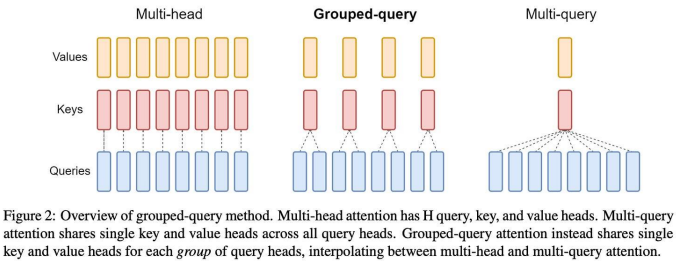
\includegraphics[width=0.6\textwidth]{pic/llama.png}
        \caption{}
    \end{figure*}
\end{frame}

\begin{frame}{Llama 2 Architecture}
    \hspace{1.65cm}
    \begin{figure*}
        \centering
        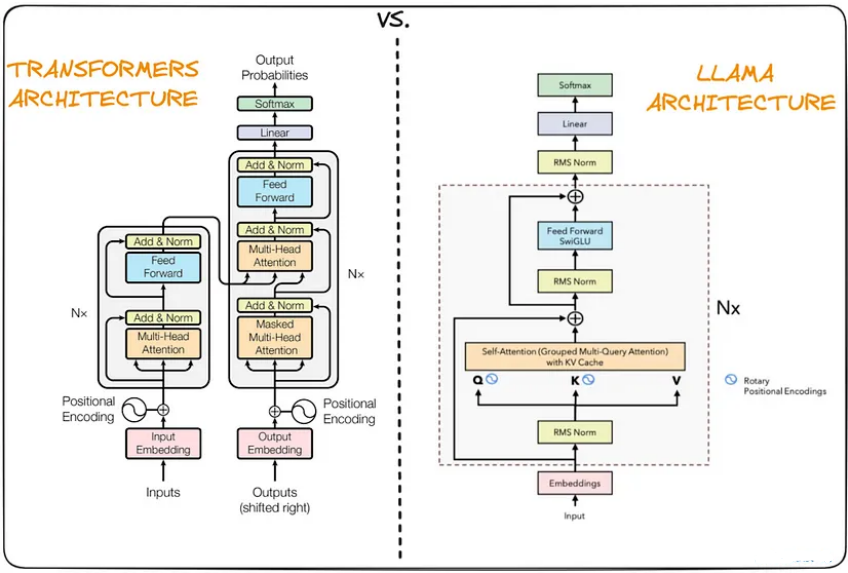
\includegraphics[width=0.75\textwidth]{pic/llamavstras.png}
        \caption{}
    \end{figure*}
\end{frame}

\begin{frame}{Training of Decoder-only LLMs – Llama 2}
    \begin{itemize}
        \item Auto-regressive Pre-training - Train to predict the next token on very large scale corpora ( ~3 trillion tokens)
        \item Instruction Fine-tuning/ Supervised Fine-tuning (SFT) - Fine-tune the pretrained model with pairs of (instruction+input,output) with large dataset and then with small high-quality dataset
        \item Safety / RLHF - Design a reward model based on human feedback and use
        policy gradient methods with the trained reward model to update LLM parameters so that outputs align with human values
    \end{itemize}
\end{frame}

\begin{frame}{RLHF}
    \hspace{2.5cm}
    \begin{figure*}
        \centering
        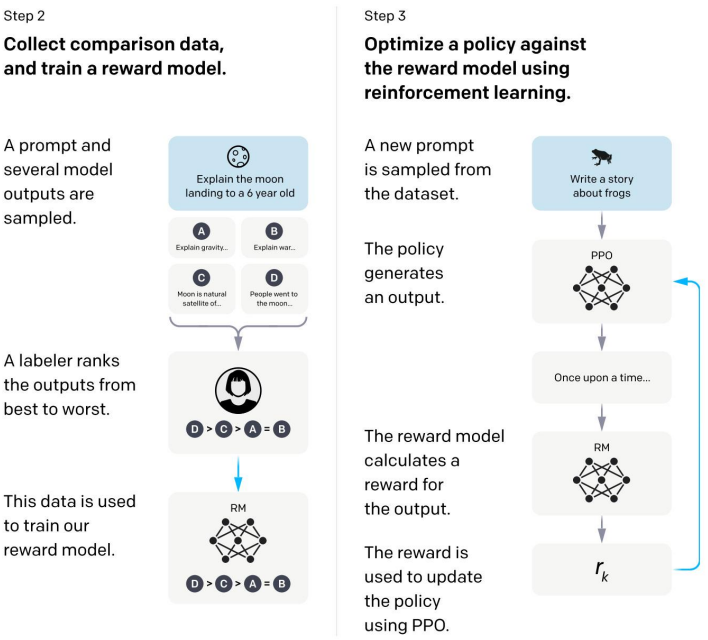
\includegraphics[width=0.6\textwidth]{pic/RLHF.png}
        \caption{}
    \end{figure*}
\end{frame}

\begin{frame}{Model Fine-tuning for RLHF}
    \hspace{1.5cm}
    \begin{figure*}
        \centering
        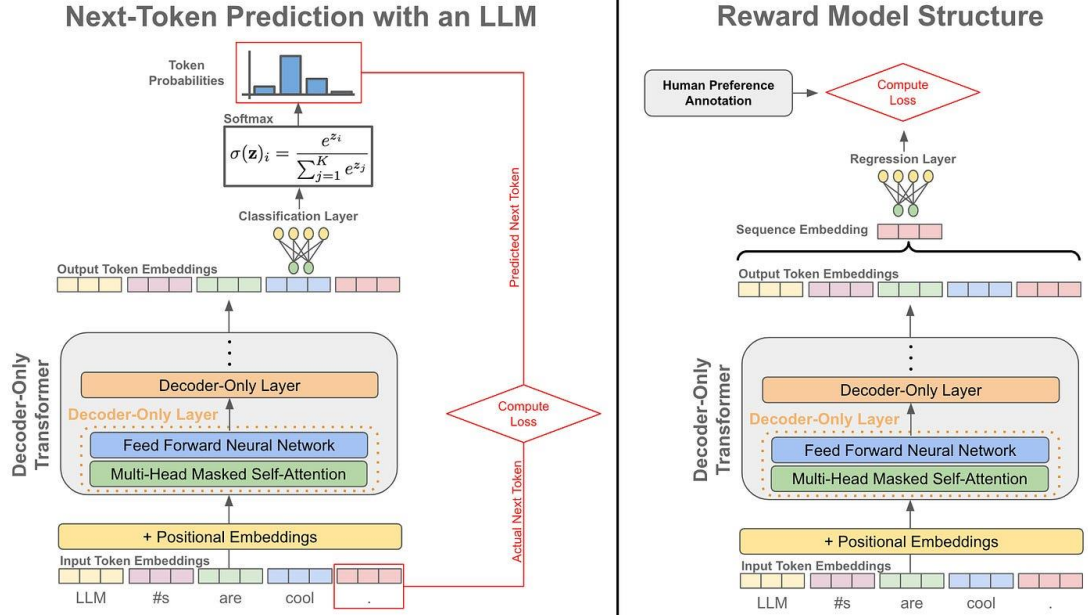
\includegraphics[width=0.8\textwidth]{pic/train RLHF.png}
        \caption{}
    \end{figure*}
\end{frame}

\section{Adaptation}
\begin{frame}{Pre-training and adaptation}
    \begin{itemize}
        \item  
            \large{Pre-training}
            \vspace{0.5cm}
            \begin{outline}
                \1 Models are initially trained on massive datasets to learn general language patterns, grammar, and common knowledge.
                \vspace{0.2cm}
                \1 The pre-trained model is further trained on a smaller, task-specific dataset to specialize in a particular application (e.g., sentiment analysis, translation).
            \end{outline}
            \vspace{0.3cm}
        \item 
            \large{Adaptation}
            \vspace{0.5cm}
            \begin{outline}
                \1 The pre-trained model is further trained on a smaller, task-specific dataset to specialize in a particular application (e.g., sentiment analysis, translation).
                \1 Fine-tuning tailors the model's responses and predictions to perform effectively on the target task.
            \end{outline}
    \end{itemize}
\end{frame}

\begin{frame}{Pre-training and adaptation}
    \begin{figure}
        \centering
        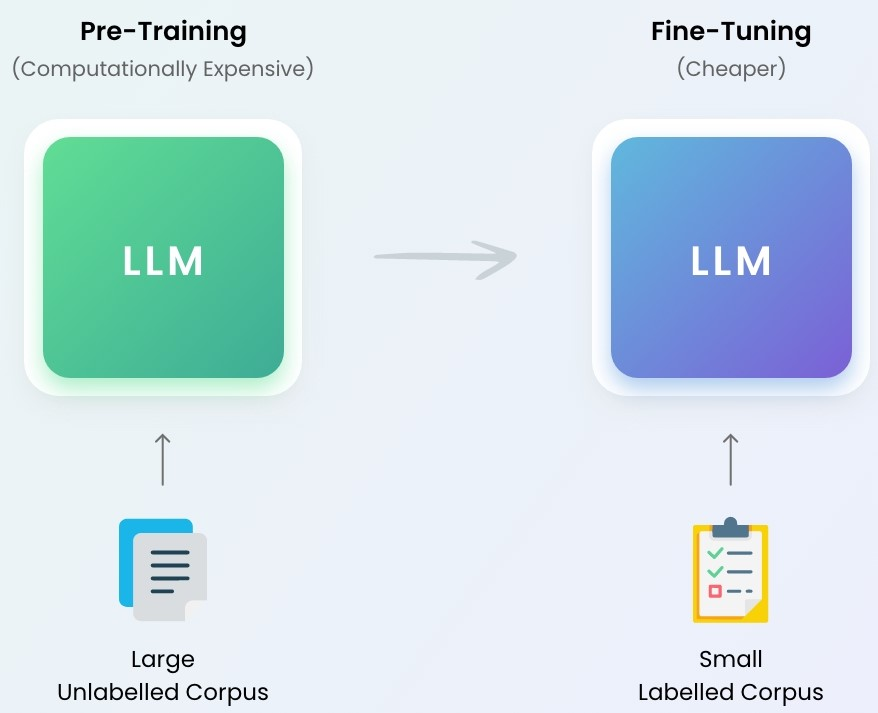
\includegraphics[width=0.5\textwidth]{pic/image.jpg}
        \caption{Overview of Model Training: Pre-training on large, unlabeled data builds foundational knowledge, while fine-tuning on smaller, labeled datasets adapts the model for specific tasks.}
    \end{figure}
\end{frame}

\section{Parameter-Efficient Fine-Tuning (PEFT)}
\begin{frame}{Parameter-Efficient Fine-Tuning (PEFT)}
    \begin{itemize}
        \item  
            \textbf{Targeted Adaptation:}
             PEFT involves fine-tuning a small subset of model parameters, allowing the pretrained model to adapt to specific tasks without retraining the entire model.
            \vspace{0.3cm}
        \item  
            \textbf{Efficiency Gains:}
              By preserving the majority of the pretrained model’s structure, PEFT significantly reduces training time, memory usage, and computational cost.
            \vspace{0.3cm}
        \item  
            \textbf{Scalability:}
              PEFT enables large language models to be applied effectively to a wide range of tasks, making it feasible to use large models in resource-constrained environments.
            \vspace{0.3cm}
    \end{itemize}
\end{frame}
    
\begin{frame}{}
    \begin{columns}
        \begin{column}{0.5\textwidth}
            \begin{itemize}
                \item  
                    \large{Fine-tuning an LLM for a specific downstream task}
                    \vspace{0.5cm}
                    \begin{outline}
                        \1 (a) illustrates vanilla fine-tuning, which requires updating the entire model, resulting in a new model for each task.
                        \vspace{0.2cm}
                        \1 (b) PEFT instead learns a small subset of model parameters for each task with a fixed base LLM. The same base model can be re-used during inference for different tasks.
                    \end{outline}
                    \vspace{0.3cm}
            \end{itemize}
        \end{column}
        \begin{column}{0.5\textwidth}
            \begin{figure}
                \centering
                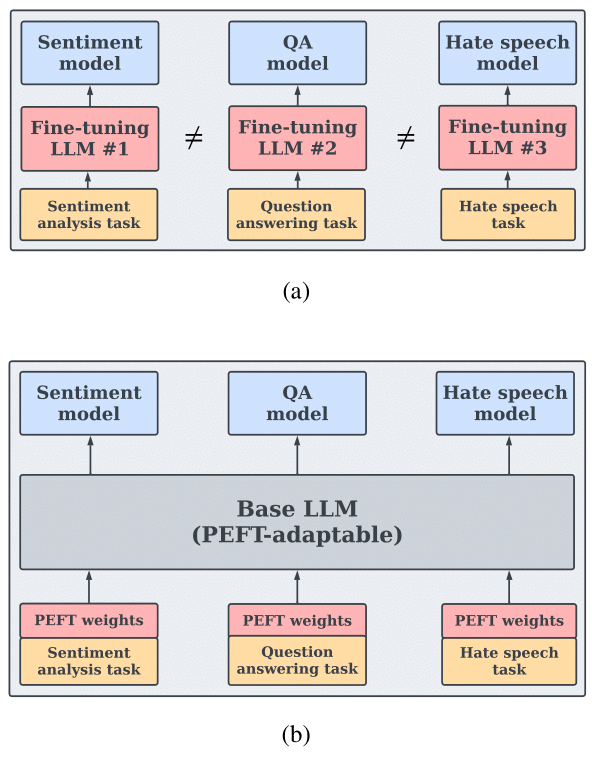
\includegraphics[width=0.75\textwidth]{pic/PEFTvsFT.png}
            \end{figure}
        \end{column}
    \end{columns}
\end{frame}

\subsection{Fine-Tuning the Top Layers Only}
\begin{frame}{Fine-Tuning the Top Layers Only}
    \begin{columns} % Begin the columns environment

        % First column for text
        \begin{column}{0.5\textwidth}
            \begin{itemize}
                \item  
                    \textbf{PEFT Baseline Efficiency:}
                     Freeze parameters except top K layers, reducing computation and memory usage.
                    \vspace{0.3cm}
                \item  
                    \textbf{Flexible Application:}
                      Can be applied to most deep neural networks for efficient fine-tuning.
                    \vspace{0.3cm}
            \end{itemize}
        \end{column}

        % Second column for the image
        \begin{column}{0.5\textwidth}
            \begin{figure}
                \centering
                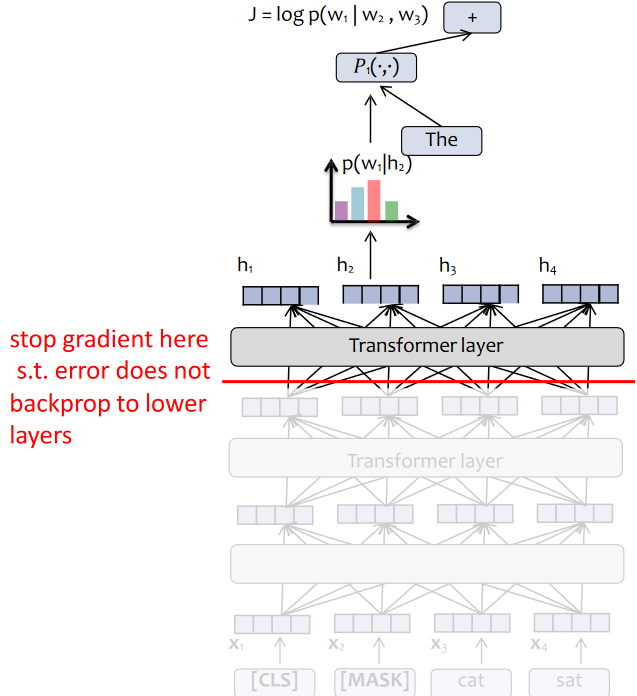
\includegraphics[width=0.85\textwidth]{pic/last layer.PNG}
            \end{figure}
        \end{column}

    \end{columns}
\end{frame}

\subsection{Adapters}
\begin{frame}{Adapters}
    \begin{columns} % Begin the columns environment

        % First column for text
        \begin{column}{0.5\textwidth}
            \begin{itemize}
                \item  
                    \textbf{Adapters: }
                     New modules inserted between layers of a pre-trained model, with the original model weights fixed.
                    \vspace{0.3cm}
                \item  
                    \textbf{Training Efficiency: }
                      Only adapter modules are tuned, initialized to ensure their output resembles that of the original model.
                    \vspace{0.3cm}
            \end{itemize}
        \end{column}

        % Second column for the image
        \begin{column}{0.5\textwidth}
            \begin{figure}
                \centering
                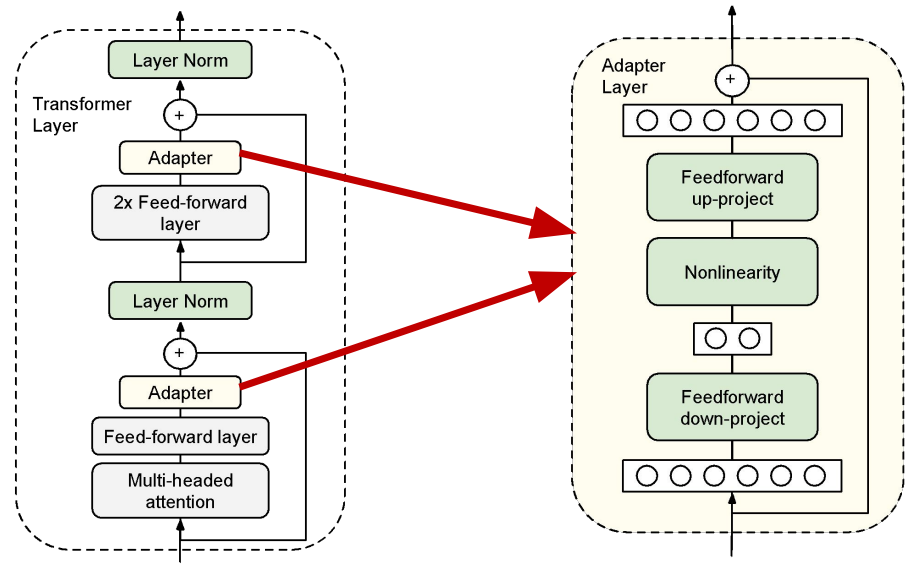
\includegraphics[width=1.04\textwidth]{pic/Adaptor.PNG}
            \end{figure}
        \end{column}

    \end{columns}
\end{frame}

\begin{frame}{Adapters}
    \begin{columns} % Begin the columns environment

        % First column for text
        \begin{column}{0.5\textwidth}
            \begin{itemize}
                \item  
                    \textbf{Adapter Design: }
                     Feedforward layer with one hidden layer and a residual connection.
                    \vspace{0.3cm}
                \item  
                    \textbf{Bottleneck Architecture: }
                     Input and output dimensions are $d$, with a reduced dimension $r$ in the middle.
                    \vspace{0.3cm}
                \item  
                    \textbf{Initialization: }
                     Near-identity initialization with a skip connection and near-zero weights.
                    \vspace{0.3cm}
            \end{itemize}
        \end{column}

        % Second column for the image
        \begin{column}{0.5\textwidth}
            \begin{figure}
                \centering
                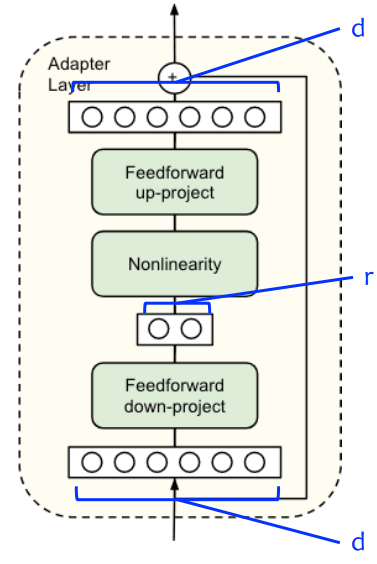
\includegraphics[width=0.68\textwidth]{pic/Adaptor 2.PNG}
            \end{figure}
        \end{column}

    \end{columns}
\end{frame}
\begin{comment}
\begin{frame}{Compacters}
            \begin{itemize}
                \item  
                    \textbf{Compacters: }
                     are an extension of adapters which aim to make the technique even more efficient.
                    \vspace{0.1cm}
                \item  
                     Adapters are standard fully connected layers.
                     \vspace{0.2cm}
                    \begin{outline}
                        \1 Linear project to lower dimension followed by nonlinearity, followed by projection back up to original dimension.
                        \vspace{0.1cm}
                        \1 \(y = \boldsymbol{W_2} GELU(\boldsymbol{W_1x} + \boldsymbol{b_1}) + \boldsymbol{b_2}\)
                    \end{outline}
                    \vspace{0.1cm}
                \item  
                     The compacter replaces the fully connected layer with a parameterized hypercomplex multiplication layer.
                     \vspace{0.2cm}
                    \begin{outline}
                        \1Each $\boldsymbol{W}$ is learned as a sum of $n$ Kronecker products.
                        \vspace{0.1cm}
                        \1 $n$ is a user-specified hyperparameter.
                    \end{outline}
                    \vspace{0.1cm}
                \item 
                    Compacters reduce the number of parameters in the adapter layer to $\frac{1}{n}$ without harming the performance.
            \end{itemize}
\end{frame}

\begin{frame}{Compacters}
    \begin{figure}
        \centering
        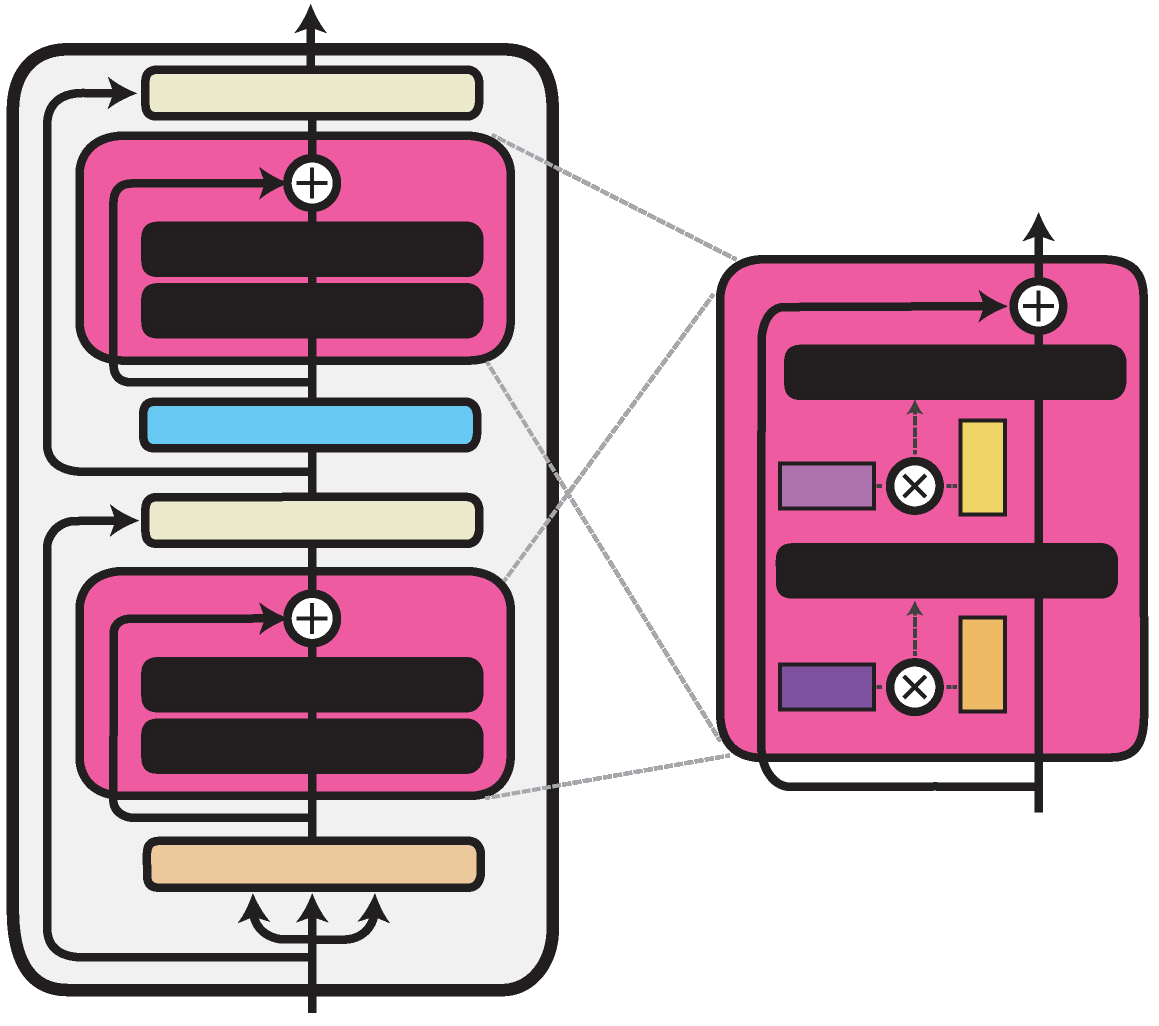
\includegraphics[width=0.6\textwidth, height=0.65\textheight]{pic/compacter.png}
        \caption{The compacter replaces the linear down and up projection of the bottleneck adapter with a phm layer. The phm layer obtains its weights by computing the kronecker product of two smaller matrices.}
    \end{figure}
\end{frame}
\end{comment}
\subsection{Bias-terms Fine-tuning (BitFit)}
\begin{frame}{BitFit}
    \begin{columns} % Begin the columns environment

        % First column for text
        \begin{column}{0.5\textwidth}
            \begin{itemize}
                \item  
                    \textbf{Bias Fine-Tuning: }
                     Only fine-tune the bias terms and final classification layer, reducing the number of parameters updated (<1\% of the model).
                    \vspace{0.3cm}
                \item  
                    \textbf{Implementation: }
                      Use a custom optimizer to fine-tune only the bias parameters by selecting them from the model’s named parameters, but this approach may fail with large models.
                    \vspace{0.3cm}
                \item Fail when model size is large
            \end{itemize}
        \end{column}

        % Second column for the image
        \begin{column}{0.5\textwidth}
            \begin{itemize}
                \item  
                    Recall the equations for multi-head attention
                    \[
                    Q^{m,\ell}(x) = W_q^{m,\ell} x + b_q^{m,\ell}
                    \]
                    \[
                    K^{m,\ell}(x) = W_k^{m,\ell} x + b_k^{m,\ell}
                    \]
                    \[
                    V^{m,\ell}(x) = W_v^{m,\ell} x + b_v^{m,\ell}
                    \]
                    \vspace{0.3cm}
                \begin{outline}
                    \1 \( \ell \) is the layer index
                    \1 \( m \) is the attention head index
                    \1 Only the bias terms are updated.
                \end{outline}
                    \vspace{0.3cm}
            \end{itemize}
        \end{column}

    \end{columns}
\end{frame}

\subsection{Reparametrization}
\begin{frame}{LoRA}
    \begin{columns}

        \begin{column}{0.5\textwidth}
            \begin{itemize}
                \item  
                    \textbf{Key Idea:} Keep the original pretrained parameters \( \boldsymbol{W_0} \) fixed and learn an additive modification \( \Delta \boldsymbol{W} \) via low-rank decomposition \( \Delta W = BA \), where \( \boldsymbol{BA} \) has rank \( r \), much smaller than \( k \) and \( d \).

                \item  
                    \textbf{LoRA Linear Layer:} The modification \( \Delta W = BA \) is added to the original linear transformation, where \( \boldsymbol{A} \) and \( \boldsymbol{B} \) have much smaller dimensions than the original weight matrix \( \boldsymbol{W_0} \).
            \end{itemize}
        \end{column}

        \begin{column}{0.5\textwidth}
            \begin{figure}
            \centering
            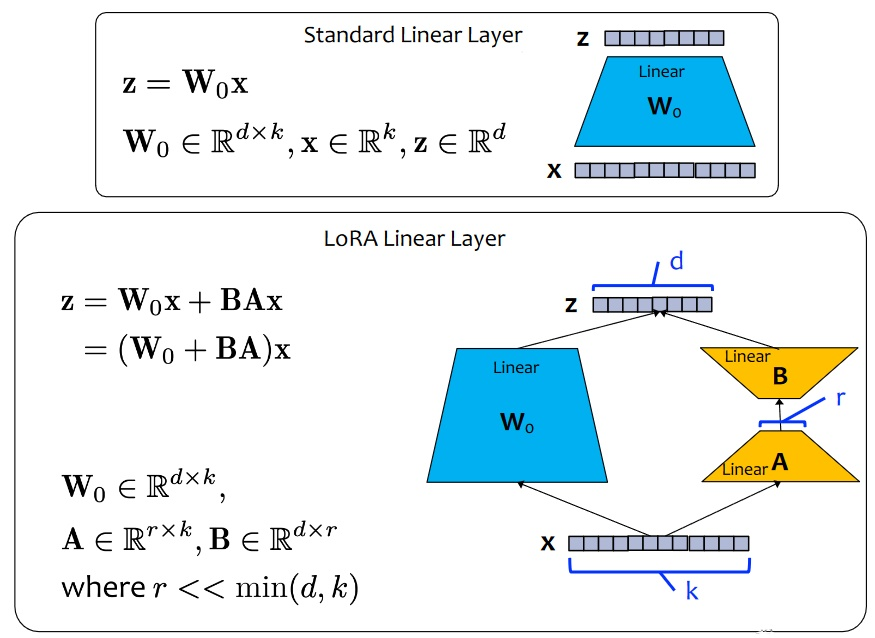
\includegraphics[width=0.95\textwidth]{pic/LoRA.jpg}
            \end{figure}
        \end{column}

    \end{columns}
\end{frame}

\begin{frame}{LoRA}
    \textbf{Initialization}
    \begin{itemize}
        \item We initialize the trainable parameters:
        \[
        A_{ij} \sim \mathcal{N}(0, \sigma^2) \quad \forall i,j
        \]
        \item \( B = 0 \)
        \item Thus, at the start of fine-tuning, the parameters have their pretrained values:
        \[
        \Delta W = BA = 0
        \]
        \[
        W_0 + BA = W_0
        \]
    \end{itemize}
\end{frame}

\begin{frame}{LoRA}
    \textbf{Hot Swapping Parameters}
    \begin{itemize}
        \item \( \boldsymbol{W_0} \) and \( \boldsymbol{BA} \) have the same dimension, so we can "swap" the LoRA parameters in and out of a Standard Linear Layer.
        \item To get a Standard Linear Layer with parameters \( \boldsymbol{W} \) that includes our LoRA fine-tuning:
        \[
        W \leftarrow W_0 + BA
        \]
        \item To remove the LoRA fine-tuning from that Standard Linear Layer:
        \[
        W \leftarrow W - BA = W_0
        \]
        \item If we do LoRA training on two tasks such that the parameters \( \boldsymbol{B'A'} \) are for task 1 and \( \boldsymbol{B''A''} \) are for task 2, then we can swap back and forth between them.
    \end{itemize}
\end{frame}

\begin{frame}{LoRA}
    \begin{itemize}
        \item \textbf{LoRA Linear Layers:} LoRA linear layers can replace every linear layer in the Transformer model.
        \vspace{0.2cm}
        \item \textbf{Original Paper Focus:} The original LoRA paper specifically applies LoRA only to the attention weights (Q, K, V).
        \vspace{0.2cm}
        \item \textbf{Mathematical Formulation:} 
        \vspace{0.3cm}
        \[
        Q = LoRALinear(X; W_q, A_q, B_q)
        \]
        \[
        K = LoRALinear(X; W_k, A_k, B_k)
        \]
        \[
        V = LoRALinear(X; W_v, A_v, B_v)
        \]
    \end{itemize}
\end{frame}

\begin{frame}{QLoRA}
    \begin{figure}
        \centering
        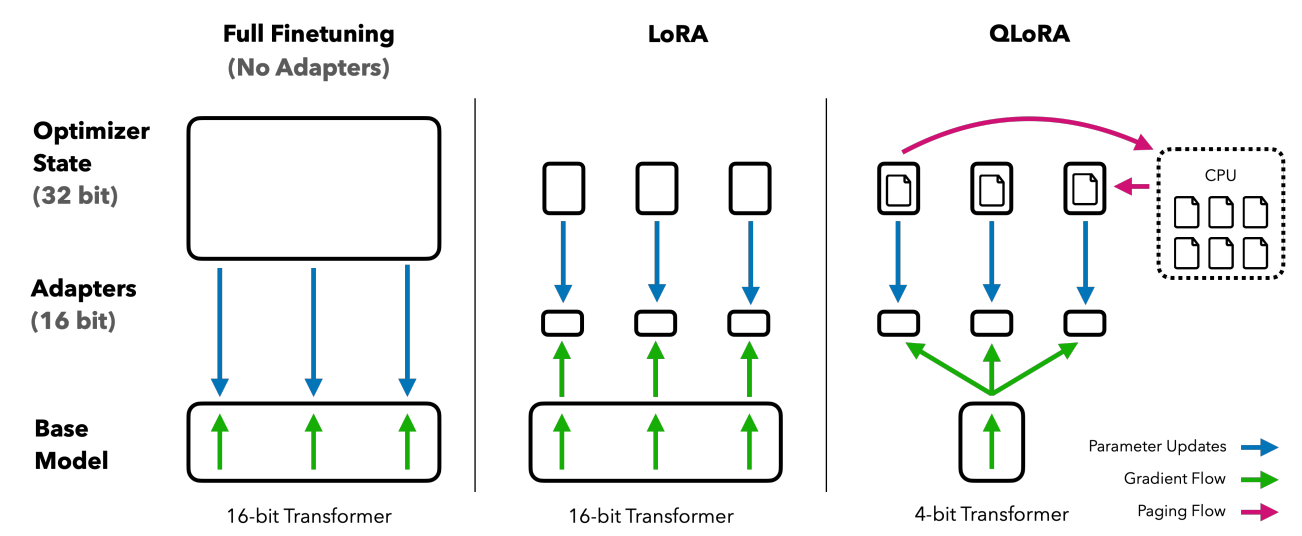
\includegraphics[width=0.75\textwidth]{pic/QLoRA.PNG}
        \caption{Different finetuning methods and their memory requirements. QLORA improves over LoRA by quantizing the transformer model to 4-bit precision and using paged optimizers to handle memory spikes.}
    \end{figure}
\end{frame}

\subsection{Prefix Tuning}
\begin{frame}{Prefix Tuning}
    \begin{itemize}
        \item Freeze all pretrained parameters and prepend trainable prefix tokens to the input and hidden activations.
        \vspace{0.2cm}
        \item The prefix is processed by the model like real words, allowing each batch element to run a different tuned model during inference.
    \end{itemize}
    \begin{figure}
        \centering
        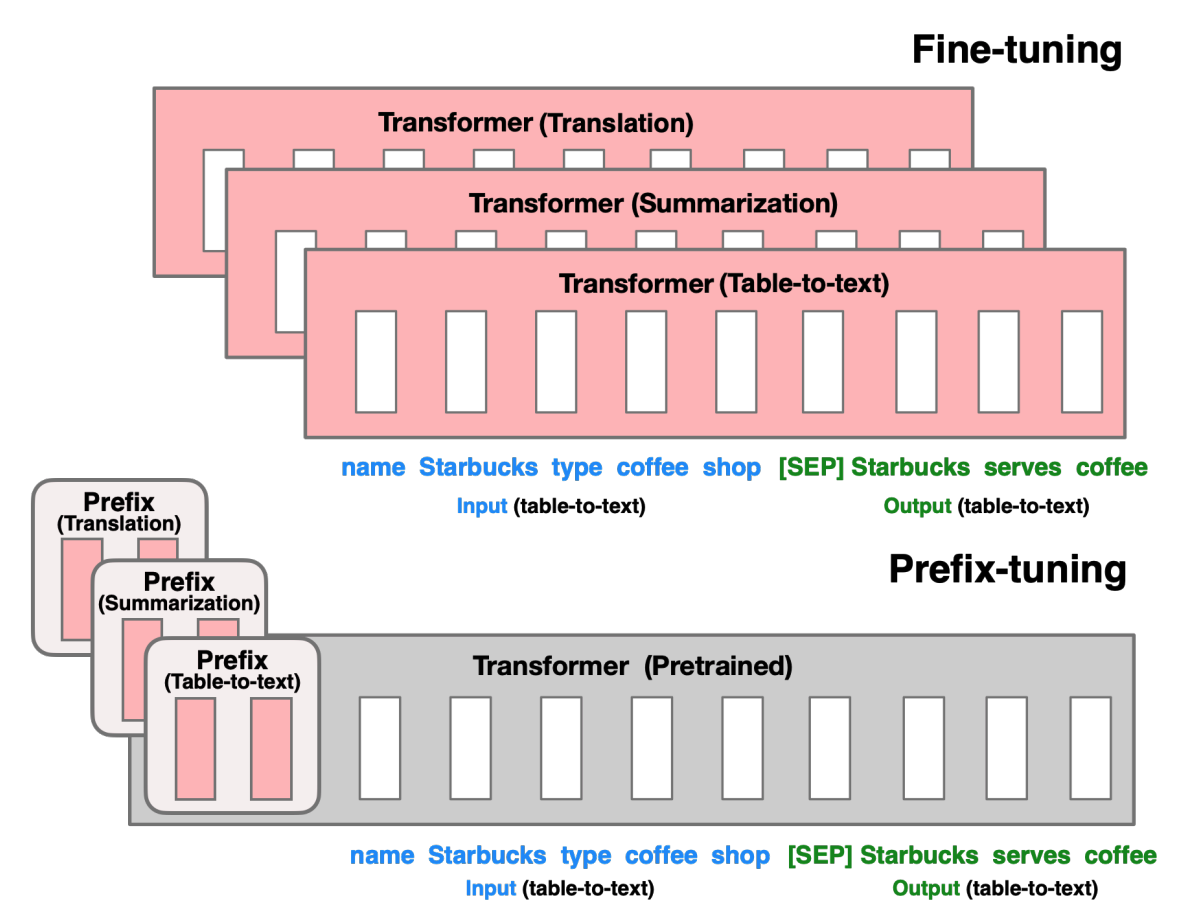
\includegraphics[width=0.43\textwidth]{pic/prefix-tuning.png}
    \end{figure}
\end{frame}

\begin{frame}{Prefix Tuning}
    \begin{figure}
        \centering
        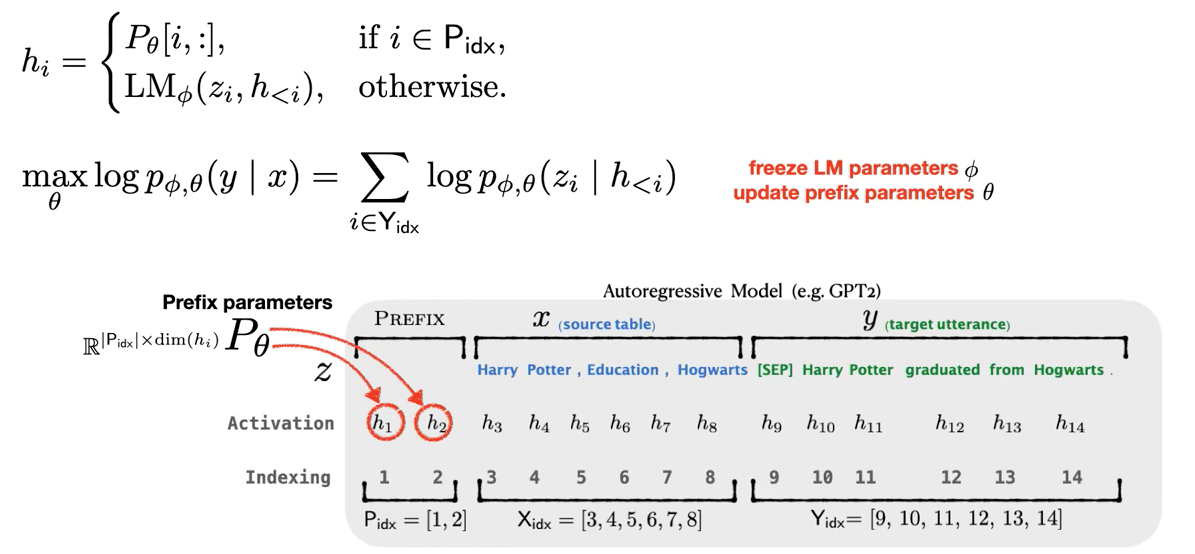
\includegraphics[width=0.9\textwidth]{pic/Prefix tuning.png}
    \end{figure}
\end{frame}

\begin{frame}{Prefix Tuning}
    \begin{columns}
        \begin{column}{0.5\textwidth}
            \textbf{Prefix Tuning with Multi-Head Attention}
            \begin{itemize}
                \item The model uses prefix tokens (\( P_k \) and \( P_v \)) along with the attention matrices (\( Q \), \( K \), \( V \)) to guide the attention mechanism in the multi-headed transformer.
                \vspace{0.3cm}
                \item The prefix tokens are processed and combined with the query, key, and value matrices (\( W_q \), \( W_k \), \( W_v \)) to form the final attention mechanism in the transformer architecture.
            \end{itemize}
        \end{column}

        \begin{column}{0.5\textwidth}
            \begin{figure}
            \centering
            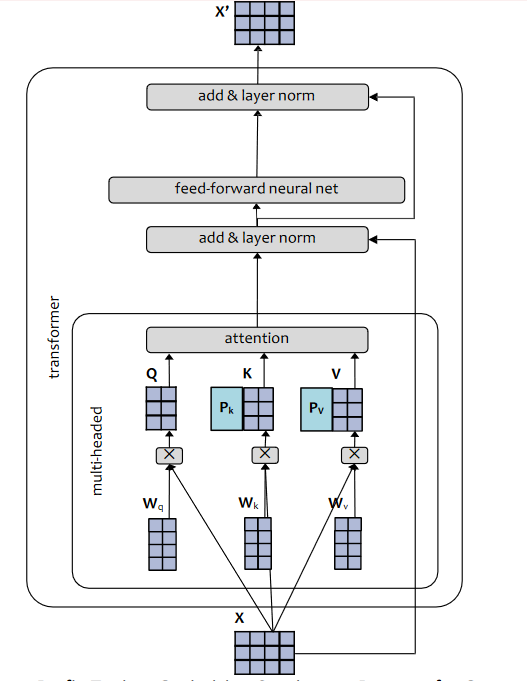
\includegraphics[width=0.7\textwidth]{pic/Prefix tuning1.PNG}
            \end{figure}
        \end{column}

    \end{columns}
\end{frame}

\begin{comment}

\section{ULMFit}
\begin{frame}{Universal Language Model Fine-Tuning Principle (ULMFit)}
    \begin{itemize}
        \item \textbf{ULMFiT Overview:} Universal Language Model Fine-tuning (ULMFiT) is a breakthrough in NLP that allows pre-trained language models to be adapted to various tasks with minimal data and improved performance.
        \vspace{0.2cm}
        \item \textbf{Key Concepts}
        \begin{outline}
            \1 \textbf{Transfer Learning:} Utilizes knowledge from one task to improve performance on related tasks.
            \vspace{0.1cm}
            \1 \textbf{Language Model Pre-training:} The model is pre-trained on large text corpora to understand general language structure before task-specific fine-tuning.
            \vspace{0.1cm}
            \1 \textbf{Discriminative Fine-Tuning:} Different layers of the model are fine-tuned at varying rates to prevent catastrophic forgetting and improve task adaptation.
            \vspace{0.1cm}
            \1 \textbf{Gradual Unfreezing:} Fine-tuning begins with the top layers, gradually unfreezing earlier layers to retain general language knowledge.
            \vspace{0.1cm}
            \1 \textbf{Slanted Triangular Learning Rates:} Adjusts learning rate by first increasing it and then slowly decreasing, optimizing fine-tuning.
            \vspace{0.1cm}
        \end{outline}
    \end{itemize}
\end{frame}

\begin{frame}{Universal Language Model Fine-Tuning Principle (ULMFit)}
    \begin{figure}
        \centering
        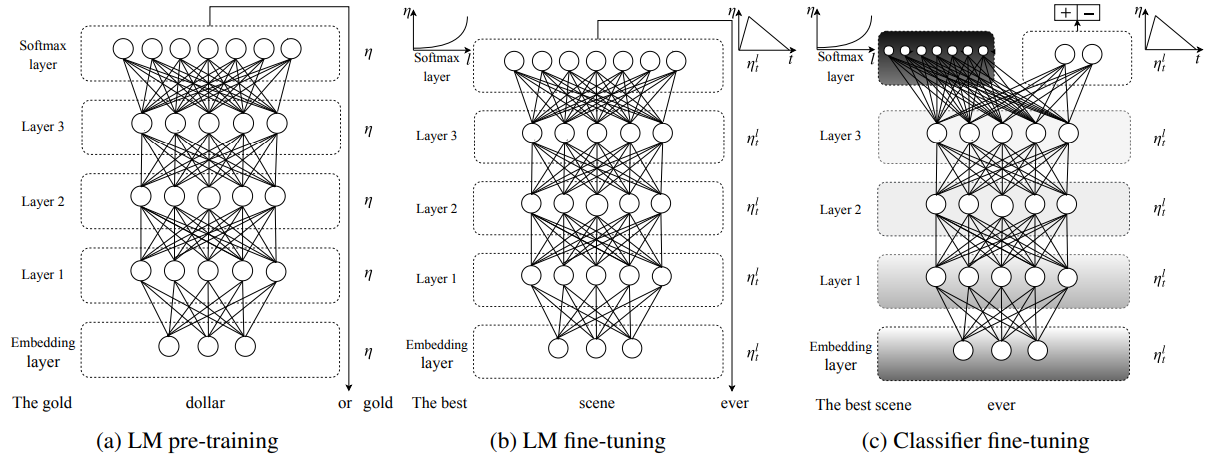
\includegraphics[width=0.85\textwidth]{pic/ULMFit.PNG}
        \caption*{\fontsize{6}{7}\selectfont
        ULMFiT consists of three stages: a) The LM is trained on a general-domain corpus to capture
        general features of the language in different layers. b) The full LM is fine-tuned on target task data using
        discriminative fine-tuning (‘Discr’) and slanted triangular learning rates (STLR) to learn task-specific
        features. c) The classifier is fine-tuned on the target task using gradual unfreezing, ‘Discr’, and STLR to
        preserve low-level representations and adapt high-level ones (shaded: unfreezing stages; black: frozen).}
    \end{figure}
\end{frame}

\begin{frame}{Universal Language Model Fine-Tuning Principle (ULMFit)}
    \begin{itemize}
        \item
        \textbf{Mathematical Concepts}
        \vspace{0.3cm}
        \begin{outline}
            \1 \textbf{Neural Networks:} ULMFiT uses Long Short-Term Memory (LSTM) networks to process text sequences.
            \vspace{0.1cm}
            \1 \textbf{Embeddings:} Words are represented as vectors in a high-dimensional space, capturing semantic relationships.
            \vspace{0.1cm}
            \1 \textbf{Gradient Descent:} Optimization method used to minimize errors by adjusting model parameters.
            \vspace{0.1cm}
            \1 \textbf{Learning Rate:} The learning rate is dynamically adjusted during training to optimize learning speed and accuracy.
            \vspace{0.1cm}
        \end{outline}
    \end{itemize}
\end{frame}
\end{comment}

\section{References}

\begin{frame}{Contribution}
    \begin{itemize}
        \item \textbf{These slides were prepared with contributions from:}
        \begin{outline}
            \1 Amirhossein Akbari
        \end{outline}
    \end{itemize}
\end{frame}


\begin{frame}
    \begin{center}
        {\Huge Any Questions?}
    \end{center}
\end{frame}

\end{document}